\documentclass[review]{article}
\usepackage[utf8]{inputenc}
\usepackage{biblatex}
\usepackage{amsmath}
\usepackage{algorithm}
\usepackage{algpseudocode}
\usepackage[hidelinks]{hyperref}
\usepackage{multicol}
\usepackage{authblk}
\usepackage{multirow}
\usepackage{mathtools}
\usepackage{float}
\usepackage{multicol}
\usepackage{graphicx}
\restylefloat{table}
\usepackage{caption}
\usepackage{subcaption}
\usepackage{caption, floatrow}
\usepackage{mathrsfs}
\usepackage{hyperref}
\usepackage{epstopdf}
\usepackage[margin=0.5in]{geometry}
\addbibresource{biblio.bib}

\renewcommand{\algorithmicrequire}{\textbf{Input:}}
\renewcommand{\algorithmicensure}{\textbf{Output:}}
\newtheorem{definition}{Definition}


\newtheorem{lemma}{Lemma}
\newtheorem{sublemma}{Lemma}[lemma]
\title { \raggedright Fast Point Cloud Sampling Network}
\author[a]{ \raggedright Tianxin Huang}
\author[a,*]{ Yong Liu \footnote{Corresponding Author}}
\author[a,b]{Jie Liang}
\affil[a]{ \raggedright Laboratory of Advanced Perception on Robotics and Intelligent Learning, College of Control Science and Engineering, Zhejiang University, Hangzhou, China}
\affil[b]{ \raggedright Beijing Institute of Mechanical and Electrical Engineering, Beijing, China}
\date{}



\begin{document}

\maketitle
\begin{multicols}{2}

\begin{abstract}

The increasing number of points in 3D point clouds has brought great challenges for subsequent algorithm efficiencies. Down-sampling algorithms are adopted to simplify the data and accelerate the computation.

\end{abstract}

\section{Introduction}
Existing works \cite{lang2020samplenet}-\cite{qi2017pointnet} often use random sampling and the farthest point sampling(FPS) to down-sample the cloud points.\\
The differences between our work and former learning-based works are presented in Fig:\ref{fig:three_graphs}
The discrepancy between progress-net and our method is
presented in Fig:\ref{fig:three_graphs}-(b) and (c).

\begin{figure}[H]
     \centering
     \begin{subfigure}[b]{0.6\textwidth}
         \centering
         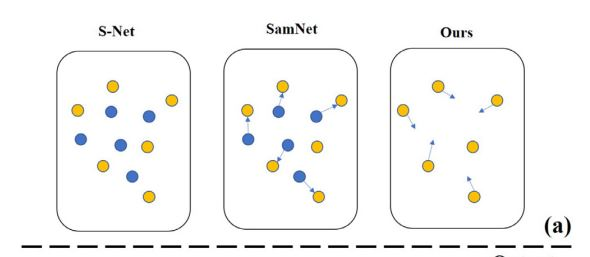
\includegraphics[width=0.6\textwidth]{pic1.jpg}
        
     \end{subfigure}
     
     \begin{subfigure}[b]{0.6\textwidth}
         \centering
         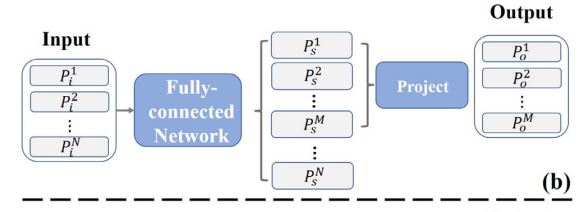
\includegraphics[width=0.6\textwidth]{pic2.jpg}
         
     \end{subfigure}
    
     \begin{subfigure}[b]{0.6\textwidth}
         \centering
         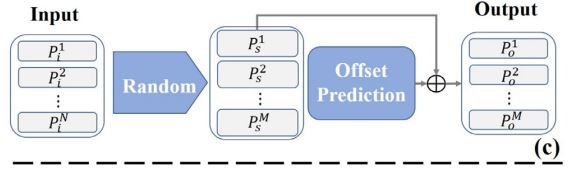
\includegraphics[width=0.6\textwidth]{pic3.jpg}
         
     \end{subfigure}
        \caption{(a) shows the differences between learning-based sampling strategies, while
(b) and (c) present the discrepancy between progress-net and our method in multiresolution sampling.}
        \label{fig:three_graphs}
    \end{figure}



\section*{}
Our
contributions can be summarized as:
\begin{itemize}
  \item We propose a novel learning-based point cloud sampling
framework named fast sampling network (FPN) by driving existing randomly sampled points to better positions;

  \item We introduce a hybrid training strategy to help FPN adapt to
different sampling resolutions by randomly introducing selecting the resolution of initial points during training;
  
\end{itemize}
\end{multicols}
\section{Methodology}
\subsection{Basic Pipeline}
The basic pipeline of FPN is presented in Fig. \ref{fig:pic4}. We aggregate
global features from the input points with a set of multilevel perceptions (MLPs) and Max Pooling following PointNet \cite{qi2017pointnet}.
\subsection*{}
\begin{figure}[H]
    \centering
    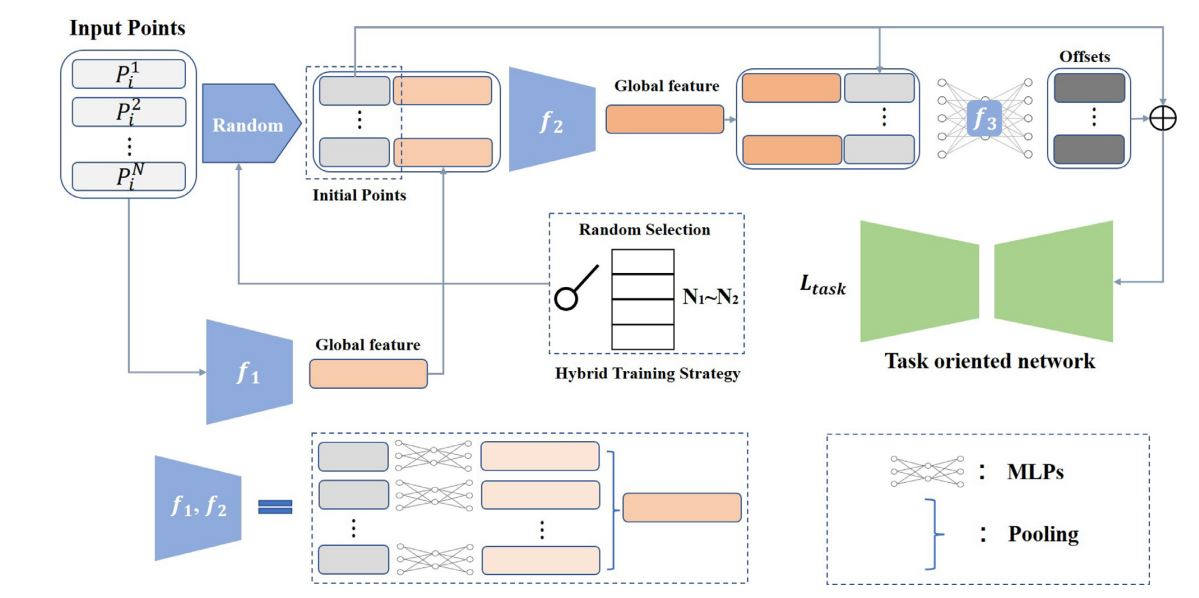
\includegraphics{pic4.jpg}
    \caption{The whole pipeline of FPN. The + denotes element-wised addition. f1 and f2 aggregate features by MultiLayer Perceptrons(MLPs) and pooling}
    \label{fig:pic4}
\end{figure}

\subsection{Hybrid Training Strategy}
The achievement of HTS is presented as Algorithm \ref{alg:cap}.
\subsection{Loss function}
The range constraint can be presented as:
\begin{equation}
    \mathcal{L}_{rc}=\frac{1}{N}\displaystyle\sum\limits_{}\parallel S_0 - S_i\parallel_2
\end{equation}
For reconstruction related tasks, it may be Chamfer Distance or Earth Mover Distance \cite{lang2020samplenet} defined as:
\begin{equation}
    \mathcal{L}_{task}=\mathcal{L}_CD(S_1,S_2)\\
    =\frac{1}{2}
(
    \frac{1}{\mid S_1 \mid}\sum_{x\in S_1} min_{y\in S_2} \parallel x-y \parallel_2 +
    \frac{1}{\mid S_2 \mid}\sum_{x\in S_2} min_{y\in S_1} \parallel x-y \parallel_2
)
\end{equation}
or
\begin{equation}
    {\mathcal{L}}_{task}=\min_\phi : S_1\longrightarrow S_2 \frac{1}{\lvert S_1 \lvert} \displaystyle\sum\limits_{x\in S_1} 
\parallel x-\phi(x)\parallel_2
\end{equation}
            
where S1 and S2 are input and output.{$\phi$}  is a bijection from S1 to S2.

\newpage

\begin{multicols}{2}




\section{Experiments}
\subsection*{Table1}

The number of neurons in networks. {$f_1$}, {$f_2$}, {$f_3$} are modules in Fig. \ref{fig:pic4}.
\newline
\begin{tabular}{l l l l}
    \hline
    \textbf{ } & $f_1$ & $f_2$ & $f_3$\\ 
    \hline
    MLPs & (128,256,256) & (128,256,256) & (128,128,3)\\
    \hline
\end{tabular}
\label{tab:Table1}




\subsection*{Table2}
The comparison on optimal clustering.\\
\\
\begin{tabular}{cllll}
\hline
Center                                  & Iterations & 1             & 10            & 100           \\
\hline
\multicolumn{1}{c}{\multirow{2}{*}{16}} & FPS        & 2.43          & 2.00          & 1.98          \\
\multicolumn{1}{c}{}                    & Ours       & \textbf{2.16} & \textbf{1.98} & \textbf{1.96} \\
\multirow{2}{*}{32}                     & FPS        & 1.20          & 1.02          & 1.00          \\
                                        & Ours       & \textbf{1.11} & \textbf{1.00} & \textbf{1.00}\\
                                        \hline
\label{tab:Table2}
\end{tabular}

\\
VIDIA
2080ti GPU with a 2.9GHZ i5-9400 CPU based on Tensorflow. The
hyper-parameter  is tuned on the validation split of ShapeNet.
Detailed network structures are shown in Table \ref{tab:Table1}.

\subsection{Discussion about clustering}
Except down-stream tasks such as reconstruction or recognition, down-sampled points can also be adopted as the initial clustering centers. \\
The results are presented in Table \ref{tab:Table2}.
\end{multicols}

\section*{}

\begin{algorithm}
\caption{Training with Hybrid Training Strategy}
\label{alg:cap}
\begin{algorithmic}
\Require{ data X, the number of iterations iter, the number of resolutions m;}
 
\For{i=1 \textbf{to} iter}                    
    \State {Select the resolution r {$prob_1,...prob_m$}
    \State {Train FPN by descending gradient:
    {$\delta_{\theta_{VPN}}$}{$\mathcal{L}_{loss}$}{$(Y_{X,r})$}
    }}
    \EndFor



\end{algorithmic}
\end{algorithm}

\section{The influence of range constraint}
The sampling efficiency is important for real-world applications. In this section, we compare the time efficiency of different.
sampling strategies under different resolutions between 64-1024.
Though random sampling is a little faster than our method, it often gets the worst results as shown in Fig. \ref{fig:fig4} and FPN outperforms commonly used sampling strategies such as FPS and SNet on task performances, while \cite{qi2019deep} it is only slower than the random
sampling. 

\begin{figure}[H]
    \centering
    \begin{subfigure}[b]{0.4\textwidth}
         \centering
         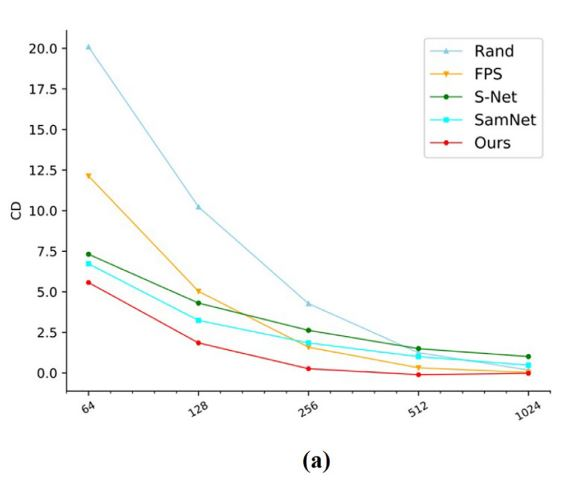
\includegraphics[width=0.6\textwidth]{pic11.jpg}
        
     \end{subfigure}
     \begin{subfigure}[b]{0.4\textwidth}
         \centering
         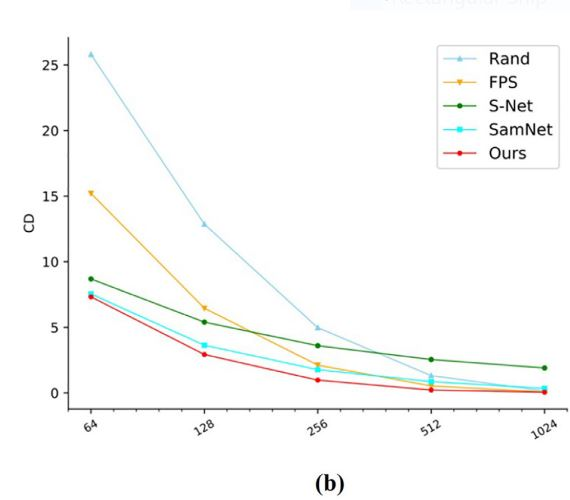
\includegraphics[width=0.6\textwidth]{pic12.jpg}
        
     \end{subfigure}
     \begin{subfigure}[b]{0.4\textwidth}
         \centering
         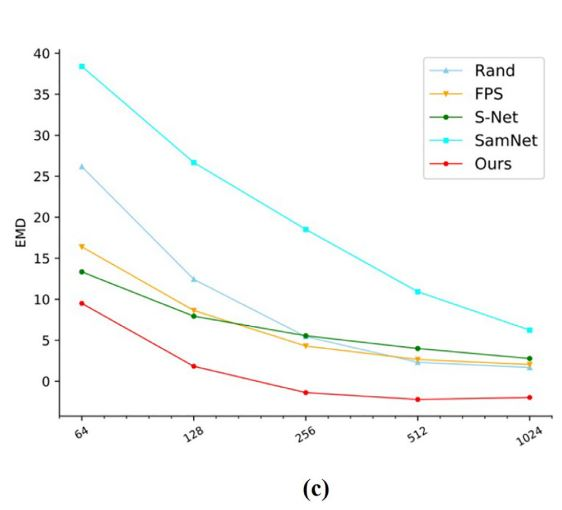
\includegraphics[width=0.6\textwidth]{pic13.jpg}
        
     \end{subfigure}
     \begin{subfigure}[b]{0.4\textwidth}
         \centering
         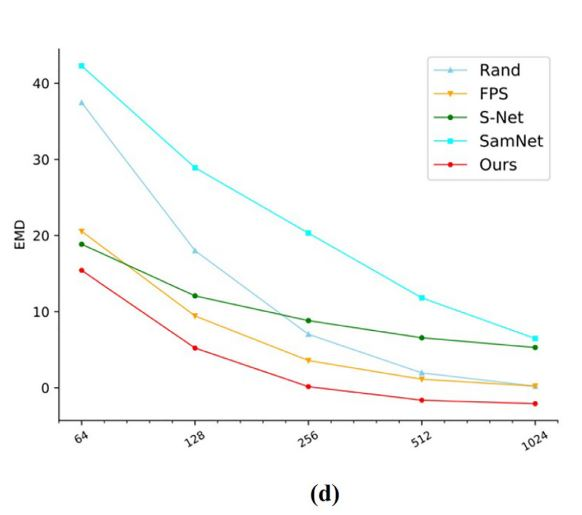
\includegraphics[width=0.6\textwidth]{pic14.jpg}
        
     \end{subfigure}
     
    \caption{Reconstruction comparisons between sampling strategies. (a) and (b) denote errors evaluated on ModelNet10 and ModelNet40 for CD-based reconstruction networks,
while (c) and (d) show performances of EMD-based reconstruction networks on ModelNet10 and ModelNet40.}
    \label{fig:fig4}
\end{figure}


\section*{Acknowledgement}
We thank all reviewers and the editor for excellent contributions. This work is supported by the Key Research and Development Project of Zhejiang Province under Grant 2021C01035.

\section*{}
\printbibliography


\end{document}
